\section[Tipos de Estadísticas]{Tipos de Variables Estadíticas}

\begin{frame}{Estimadores}
    \begin{itemize}
        \item Si el desempeño del sistema se mide mediante un parámetro $\theta$, el resultado de un conjunto de corridas de simulación será un estimador estadístico $\hat{\theta}$ de $\theta$.
        \item La precisión del estimador $\hat{\theta}$ puede ser medida por un error estándar de $\hat{\theta}$ o por un intervalo de confianza para $\theta$.
        \item El propósito del análisis estadístico es o bien estimar el error estándar o el intervalo de confianza, o bien determinar el número de observaciones requeridas para alcanzar un error estándar o intervalo de confianza de una longitud dada.
    \end{itemize}
\end{frame}

\begin{frame}{Estimadores}{Intervalos de confianza}
    \begin{itemize}
        \item El intervalo de confianza cuantifica la probabilidad de que el parámetro estadístico real (desconocido) caiga dentro de unos límites calculados con los estimadores puntuales apropiados.
        \item El intervalo de confianza es una medida de error constituida mediante un rango alrededor del estimador puntual de la forma:
        $\hat{\Theta}\pm h$, donde $h$ es denominado ancho medio (half-widht).
        %\item Podemos a través de la simulación disminuir el error haciendo más réplicas.
    \end{itemize}
\end{frame}

%\begin{frame}{Experimento de simulación}
%    \begin{itemize}
%        \item Un experimento de simulación ocurre cuando el analista fija unos parámetros de entrada para el modelo y ejecuta la simulación.
%        \item Durante la simulación, el comportamiento del sistema es observado y varias estadísticas son calculadas.
%        \item Cuando la simulación alcanza su punto de culminación, las estadísticas son resumidas en la forma de un reporte de salida.
%    \end{itemize}
%\end{frame}

%Replication
\begin{frame}{Réplicas}
    \begin{itemize}
        \item Una \textit{réplica} es la generación de una ruta muestral que representa la evolución del sistema desde sus condiciones iniciales hasta su terminación.
        \item Un experimento de simulación puede consistir en una o varias réplicas.
        \item Si hay múltiples réplicas dentro una simulación, cada una representa un camino muestral, que empieza en las mismas condiciones iniciales y es controlado por la misma configuración de parámetros.
        \item Las réplicas están sujetas a las mismas fuentes de variabilidad, de forma independiente unas de otras. 
    \end{itemize}
\end{frame}

\begin{frame}{Tipos de estadísticas}{Estadísticas dentro de las réplicas}
    \begin{itemize}
        \item Son recolectadas con base en la observación de un camino muestral e incluye las observaciones sobre entidades, cambios de estado, etc., que ocurren durante la ejecución de la corrida.
        \item Probablemente no son independientes e idénticamente distribuidas ya que se encuentran autocorrelacionadas.
        
    \end{itemize}
\end{frame}

\begin{frame}{Tipos de estadísticas}{Estadísticas entre las réplicas}
    \begin{itemize}
        \item Son recolectadas con base en la observación de los valores finales de las observaciones dentro de cada réplica, por lo tanto, se tiene una observación por cada réplica realizada.
        \item Como cada réplica es considerada independiente, las observaciones que forman la muestra entre réplicas es probable que sean independientes e idénticamente distribuidos.
    \end{itemize}
\end{frame}

\begin{frame}{Tipos de estadísticas}
    \begin{figure}
        \centering
        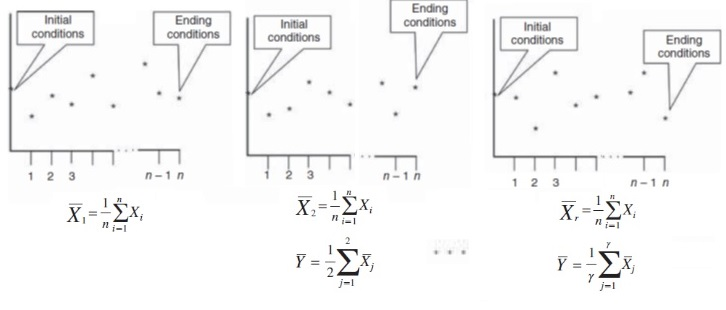
\includegraphics[width=11.5cm]{images/Statistics.jpg}
        %\caption{Caption}
        %\label{fig:my_label}
    \end{figure}
\end{frame}

\begin{frame}{Observaciones}
    \begin{itemize}
            \item Las observaciones pueden ser de dos tipos:
        \begin{itemize}
            \item \textbf{Tally}: representa una secuencia de datos que no persisten en el tiempo (tiempo en cola, número de entidades procesadas, si un cliente en particular esperó más de 10 minutos, etc.) 
            \item \textbf{Time-persistent}: representa una secuencia de valores que persisten durante un cierto tiempo, el valor se pondera por la cantidad de tiempo que persiste (promedio de entidades en cola, porcentaje de tiempo que hay cola, utilización del servidor, etc.)
        \end{itemize}
    \end{itemize}
\end{frame}